\pdfminorversion=4 
\documentclass{beamer}
\usepackage[utf8x]{inputenc}
\usepackage[T1]{fontenc}
\usepackage{lmodern}
\usepackage[english]{babel}
\usetheme{Padova}
\usepackage[font=small]{caption}
\usepackage{breqn}
\usepackage{amsmath}
\usepackage{amssymb}
\usepackage{wrapfig}
\usepackage{float}
\usepackage{graphicx}
\usepackage{booktabs}
\usepackage{pgfplots}
\usepackage{pgfplotstable}
\pgfplotsset{compat=1.9}  
\usepackage{hyperref}
\usepackage{media9}
\usepackage{siunitx}

\usepackage{caption}
\captionsetup[figure]{name=Fig}

\title{Neural Spike Digital Detector \\on FPGA}
\author{Rocco Ardino\\Alessandro Lambertini\\Alice Pagano\\Michele Puppin}
\date{}
\institute[]

\begin{document}
	
\begin{frame}
    \maketitle
\end{frame}

%%%%%%%%%%%%%%%%%%%%%%%%%%%%%%%%%%%%%%%%%%%%%%%%%%%%%%%%%%%%%%%%%%%%%%%%%%%%%%%%%%%%%%%
\begin{frame}{Introduction}
\begin{columns}
    \begin{column}{1.05\textwidth}
        \begin{itemize}
            \item Many advanced neurobiology techniques require a communication interface to analyse neural activity and to perform neural stimulation
        \end{itemize}
    \end{column}
\end{columns}
\begin{columns}
    \begin{column}{0.7\textwidth}
        \begin{itemize}
        	\item It needs advanced electronics systems composed by:
            	\begin{itemize}
            	    \item analog stages to acquire biological signals
            	    \item \textbf{advanced algorithms} to separate signals from \textbf{background noise}
            	    \item electrical stimulation stages
    	        \end{itemize}
            \end{itemize} 
    \end{column}
    \hspace{-0.6cm}
    \begin{column}{0.35\textwidth}
        \begin{figure}
            \vspace{-0.2cm}
            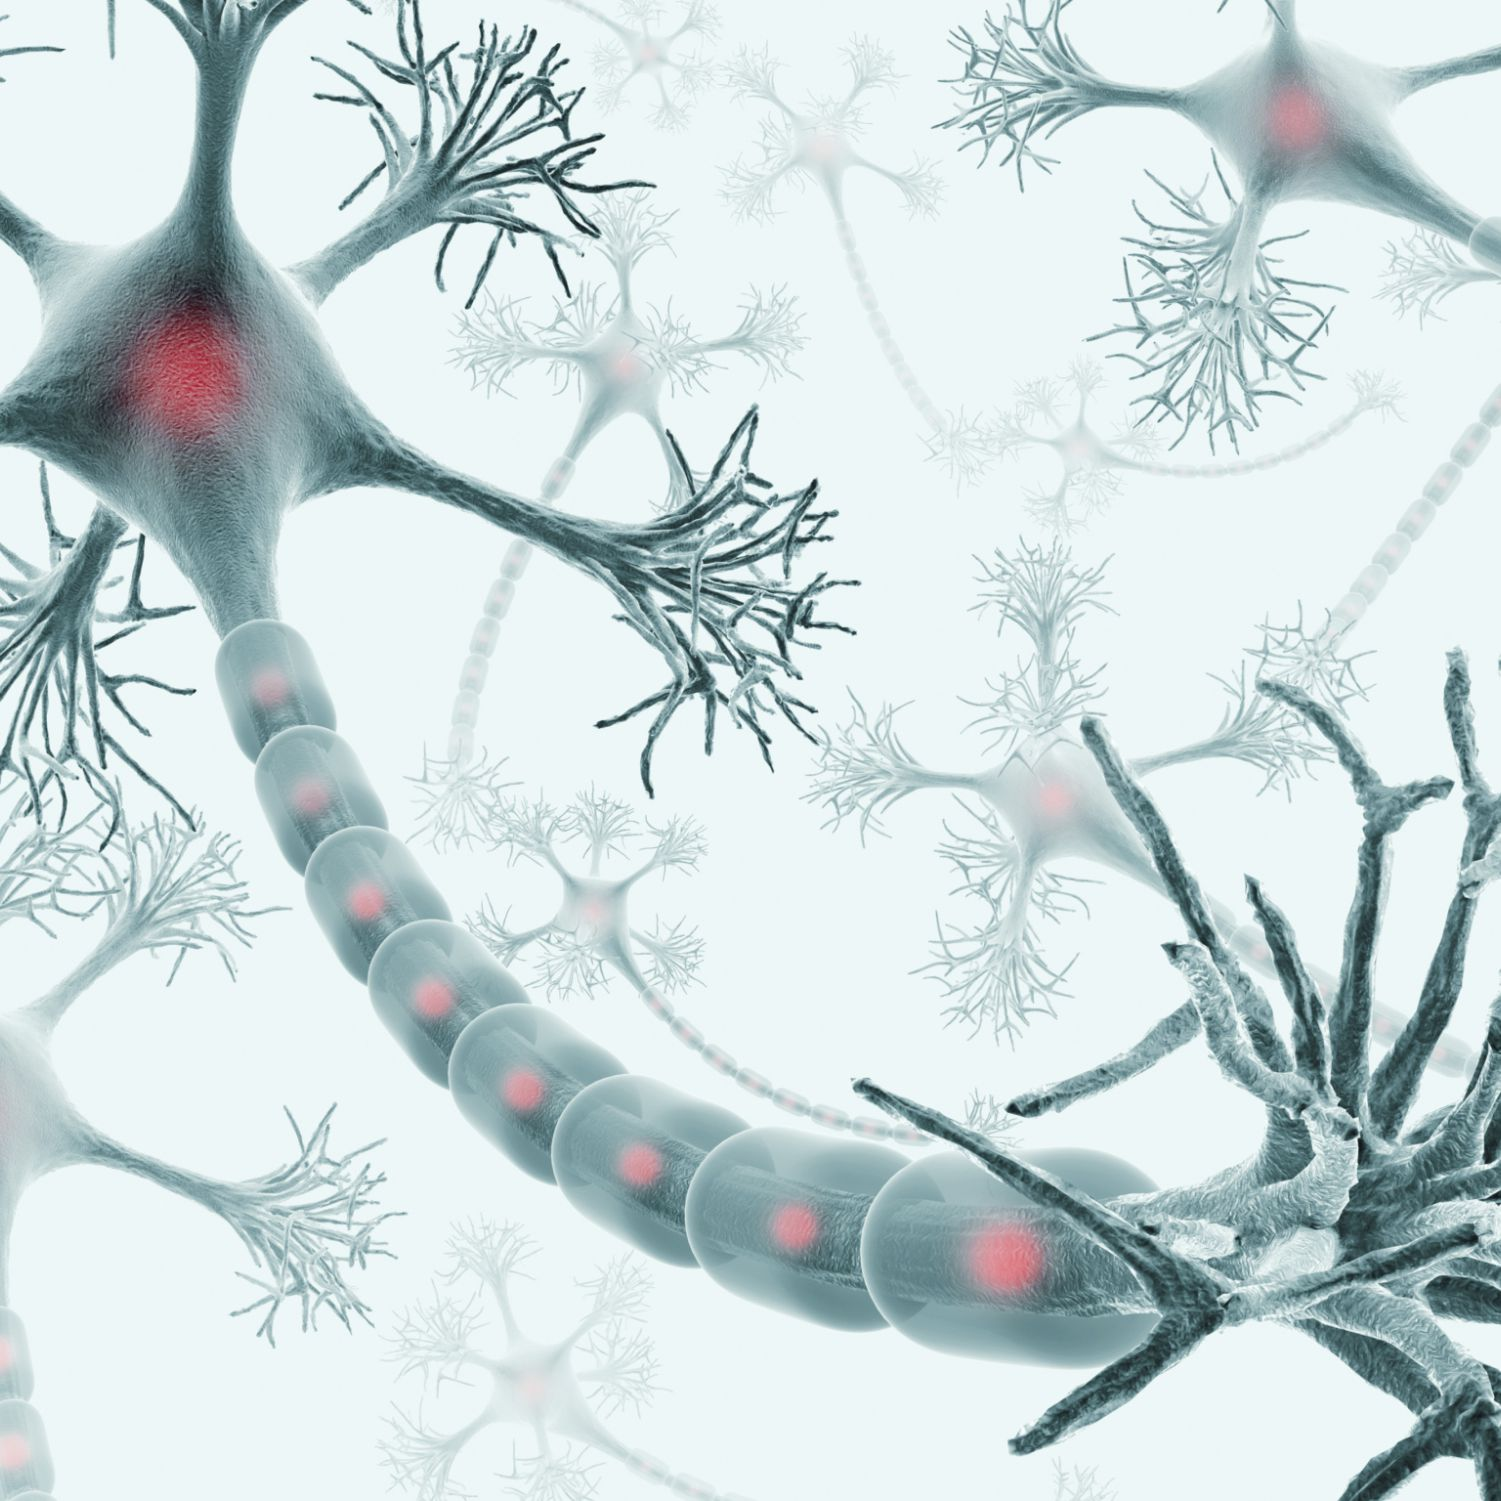
\includegraphics[width=4cm]{neur.jpg}
            \caption{Neuron cartoon}
        \end{figure}
    \end{column}
\end{columns}
\end{frame}

%%%%%%%%%%%%%%%%%%%%%%%%%%%%%%%%%%%%%%%%%%%%%%%%%%%%%%%%%%%%%%%%%%%%%%%%%%%%%%%%%%%%%%%
\begin{frame}{Neuron communication}
\vspace{-1.7cm}
\begin{columns}
    \begin{column}{0.6\textwidth}
        \begin{itemize}
            \item Neuron communication is carried out through \textbf{action potentials} (AP) $\xrightarrow{}$ trans-membrane voltage of $ 100 \: mV_{PP}$ and few $kHz$
        \end{itemize}
    \end{column}
    \begin{column}{0.4\textwidth}
        \begin{figure}
            \vspace{0.6cm}
            \hspace{-1cm}
            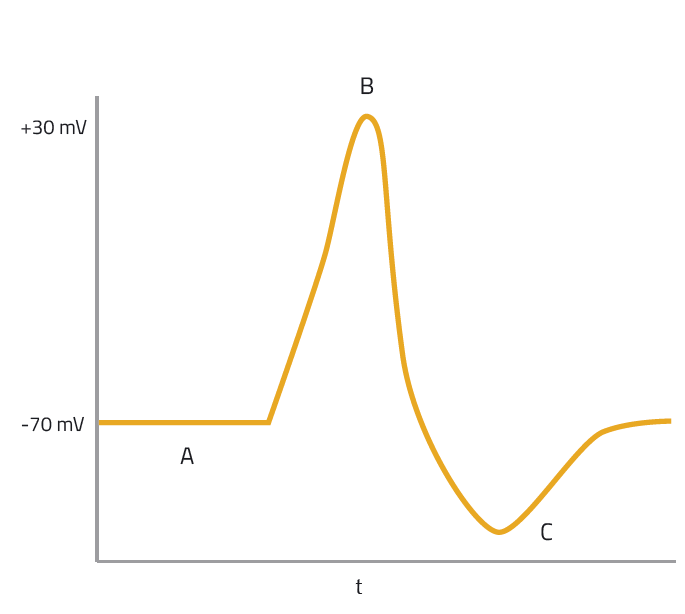
\includegraphics[width=5cm]{act_pot.png}
        	\caption{Action Potential}
        \end{figure}
    \end{column}
\end{columns}
\begin{columns}
    \begin{column}{1.1\textwidth}
        \begin{itemize}
        	\item Most common technique to observe neurons utilized needle-shaped probes that deeply penetrate the cells:
            	\begin{itemize}
            	    \item[$\checkmark$] high signal-to-noise ratio
            	    \item[$\times$] average cell life of few days
    	        \end{itemize}
            \end{itemize} 
    \end{column}
\end{columns}
\end{frame}

%%%%%%%%%%%%%%%%%%%%%%%%%%%%%%%%%%%%%%%%%%%%%%%%%%%%%%%%%%%%%%%%%%%%%%%%%%%%%%%%%%%%%%%
\begin{frame}{State-of-the-art approaches}
\begin{itemize}
    \item Minimally-invasive sensing techniques, based on \textbf{CMOS} microelectrode arrays, are state-of-the-art approaches
    \begin{itemize}
        \item[$\checkmark$] preserve cell for long time observations
        \item[$\times$] low signal-to-noise ratio
    \end{itemize}
    \item Recorded signals are improved by advanced post-processing \textbf{spike sorting algorithms} that separate relevant neural spikes from background noise
\end{itemize}
\begin{figure}
    \centering     
    \vspace{-0.4cm}
    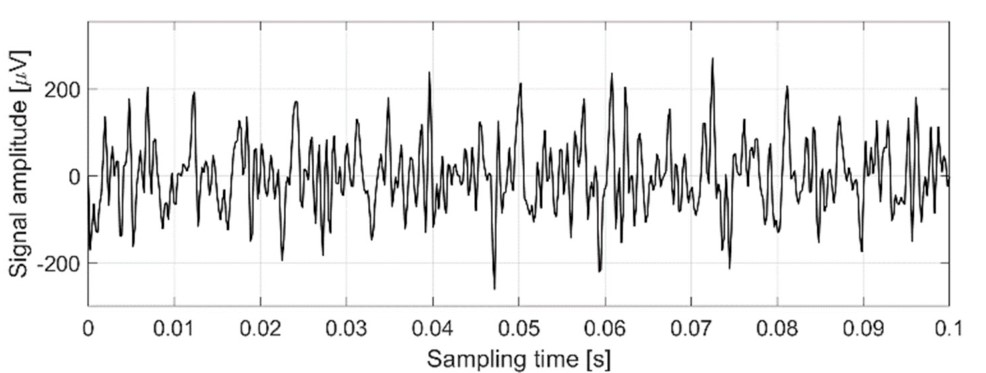
\includegraphics[width=9cm]{sig-noise.jpg}
    \vspace{-0.1cm}
    \caption{Single pixel signal time evolution}
\end{figure}
\end{frame}

%%%%%%%%%%%%%%%%%%%%%%%%%%%%%%%%%%%%%%%%%%%%%%%%%%%%%%%%%%%%%%%%%%%%%%%%%%%%%%%%%%%%%%%
\begin{frame}{Neural Spike Digital Detector (i)}
\begin{itemize}
    \item This work analyzes the \textbf{neural spike digital detector} (NSDD) hardware design
    \item An action potential detector has been implemented on a FPGA
    \item It identifies single AP signals with amplitudes around $200-600 \: \mu V$ recorded on pixels of a CMOS MEA
    \item In situ neural activity recognition greatly limits the bandwidth required to transmit data and the associated power consumption
\end{itemize}
\end{frame}

%%%%%%%%%%%%%%%%%%%%%%%%%%%%%%%%%%%%%%%%%%%%%%%%%%%%%%%%%%%%%%%%%%%%%%%%%%%%%%%%%%%%%%%
\begin{frame}{Neural Spike Digital Detector (ii)}
\begin{itemize}
    \item Neuronal cells are seeded on the CMOS MEA composed by: 
    \begin{itemize}
        \item the capacitive sensor matrix ($256 \times 384$ pixels)
        \item the electronics signal processing stages
    \end{itemize}
    \item A comunication interface forward the digitized signals from the output to the NSDD FPGA at \textbf{14.1 MS/s}.
\end{itemize}
\begin{figure}
    \centering   
    \vspace{-0.4cm}
    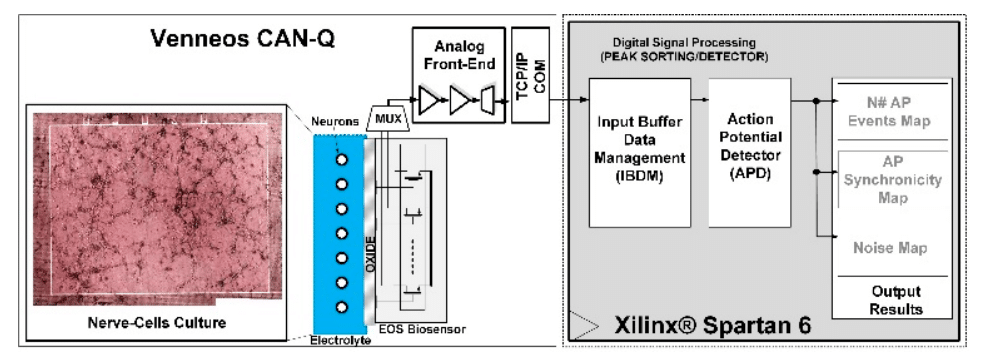
\includegraphics[width=9cm]{structure.png}
    \caption{Neuronal-cell culture experimental setup}
\end{figure}
\end{frame}

%%%%%%%%%%%%%%%%%%%%%%%%%%%%%%%%%%%%%%%%%%%%%%%%%%%%%%%%%%%%%%%%%%%%%%%%%%%%%%%%%%%%%%%
\begin{frame}{Neural Interface Noise}
\begin{itemize}
    \item Extracellular signal amplitudes are two orders of magnitude smaller than invasive techniques.
    \item Adhesion of cells to the surface increases the noise power
    \item An \textbf{accurate noise evaluation} and a proper spike detector is needed to avoid discarding most of the action potentials
\end{itemize}

\begin{figure}
    \centering    
    \vspace{-0.5cm}
    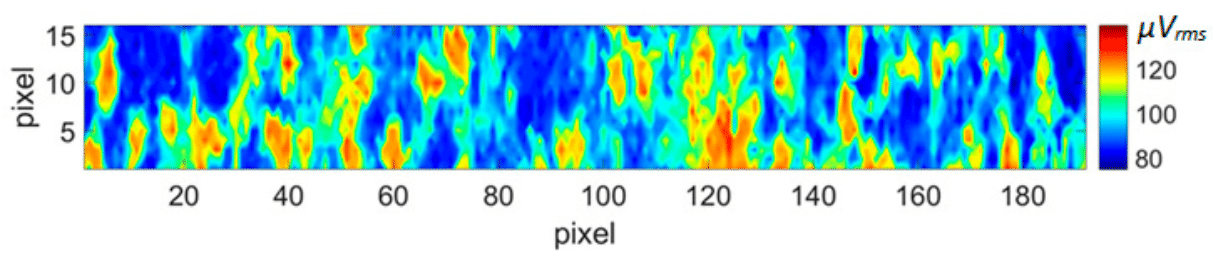
\includegraphics[width=11cm]{noise.png}
    \vspace{-0.8cm}
    \caption{Noise power spatial map}
\end{figure}
\vspace{-0.5cm}
\begin{itemize}
    \item In areas without cell exhibit the noise is $ 80 \: \mu V_{RMS}$ 
    \item In pixel beneath cell the noise is $ 120 \: \mu V_{RMS}$ 
\end{itemize}
\end{frame}

%%%%%%%%%%%%%%%%%%%%%%%%%%%%%%%%%%%%%%%%%%%%%%%%%%%%%%%%%%%%%%%%%%%%%%%%%%%%%%%%%%%%%%%
\begin{frame}{Principal Component Analysis (i)}
\begin{itemize}
    \item MEAs are characterized by high spatial and temporal resolution $\xrightarrow{}$ a single AP event can be detected:
    \begin{itemize}
        \item by 9 adjacent pixels
        \item for 3 consecutive time samples
    \end{itemize}
    \item PCA algorithm calculate the probability to detect signal in front of statistical thermal fluctuation
    \item AP is detected if:
    \begin{equation}
        \sum_{pixj=1\xrightarrow{}9} \frac{\sum_{ \{ n,n-i,n-2 \} } PIXj (n)^2 }{\sigma_{NOISE,j}^2} \geq AP\_Threshold \cong 84.6
    \end{equation}
    where $PIXj$ is the $j$-th pixels at three instants $n$, $n-i$ and $n-2$
    \item Improve global SNR at cost of a small spatial resolution reduction
\end{itemize}
\end{frame}

%%%%%%%%%%%%%%%%%%%%%%%%%%%%%%%%%%%%%%%%%%%%%%%%%%%%%%%%%%%%%%%%%%%%%%%%%%%%%%%%%%%%%%%
\begin{frame}{Principal Component Analysis (ii)}
\begin{figure}
    \centering     
    \vspace{-0.6cm}
    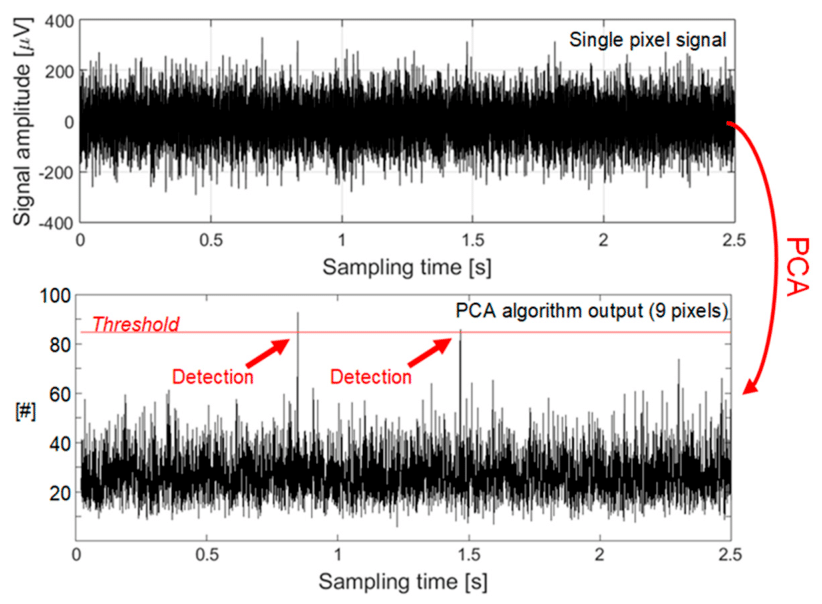
\includegraphics[width=9cm]{pca_1.png}
    \caption{PCA output compared with threshold}
\end{figure}
\end{frame}

%%%%%%%%%%%%%%%%%%%%%%%%%%%%%%%%%%%%%%%%%%%%%%%%%%%%%%%%%%%%%%%%%%%%%%%%%%%%%%%%%%%%%%%
%%%%%%%%%%%%%%%%%%%%%%%%%%%%%%%%%%%%%%%%%%%%%%%%%%%%%%%%%%%%%%%%%%%%%%%%%%%%%%%%%%%%%%%
% Lambe
%%%%%%%%%%%%%%%%%%%%%%%%%%%%%%%%%%%%%%%%%%%%%%%%%%%%%%%%%%%%%%%%%%%%%%%%%%%%%%%%%%%%%%%
%%%%%%%%%%%%%%%%%%%%%%%%%%%%%%%%%%%%%%%%%%%%%%%%%%%%%%%%%%%%%%%%%%%%%%%%%%%%%%%%%%%%%%%
\begin{frame}{Neural Spike Digital Detector on FPGA}
    The digital design for the PCA algorithm on FPGA consists of three main stages:
    \begin{itemize}
    	\item  the input-buffer-data-management (IBDM) synchronously receives the data coming from the biosensor via the TCP/IP communication interface
    	\item the action potential detector (APD), that is the digital circuit     implementing the PCA algorithm
    	\item a specific set of MATLAB functions that provide graphical representation of the on-going neural activity.
    \end{itemize}
\end{frame}

%%%%%%%%%%%%%%%%%%%%%%%%%%%%%%%%%%%%%%%%%%%%%%%%%%%%%%%%%%%%%%%%%%%%%%%%%%%%%%%%%%%%%%%
\begin{frame}{Neural Spike Digital Detector on FPGA}
To achieve the aim of real-time analysis it must be:
\begin{equation}
    \frac{\mbox{NSDD data throughput}}{\mbox{MEA sample rate}}\ge 1 \quad 
    \Rightarrow\quad f_{CLK}\ge N_{CLK}\cdot MEA_{\mbox{out}}
\end{equation}
\begin{itemize}
    \item $MEA_{out}$: MEA sample rate
    \item $f_{CLK}$: FPGA master clock frequency
    \item $N_{CLK}$: Clock cycles needed to process one sample 
\end{itemize}
\end{frame}

%%%%%%%%%%%%%%%%%%%%%%%%%%%%%%%%%%%%%%%%%%%%%%%%%%%%%%%%%%%%%%%%%%%%%%%%%%%%%%%%%%%%%%%
\begin{frame}{From neurons to PCA}
\begin{figure}
    \centering     
    \vspace{-1.6cm}
    
\includegraphics[width=10cm]{IBDM2.png}
    \caption{Data movement inside the system.}
\end{figure}
\begin{itemize}
    \item NSDD receives a stream of data from the Venneos-CAN-Q machine via an Ethernet connection using TCP/IP protocol.
    \item data are sent from the buffer to the APD stage to perform the PCA algorithm.
\end{itemize}
\end{frame}

%%%%%%%%%%%%%%%%%%%%%%%%%%%%%%%%%%%%%%%%%%%%%%%%%%%%%%%%%%%%%%%%%%%%%%%%%%%%%%%%%%%%%%%
\begin{frame}{From neurons to PCA}

    \begin{columns}
        \begin{column}{0.5\textwidth}
            \begin{figure}
                \vspace{-0.2cm}
                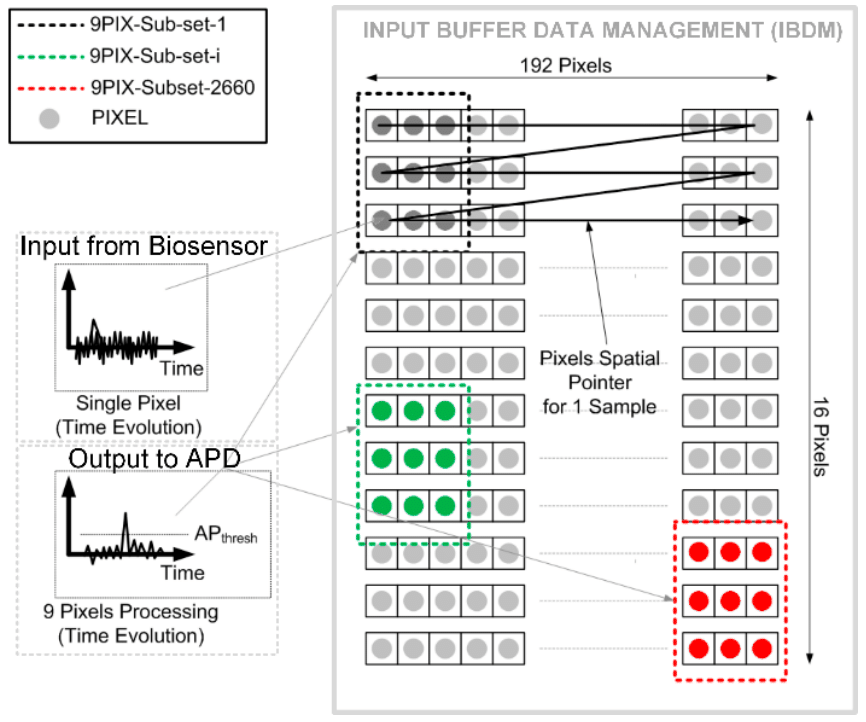
\includegraphics[width=6cm]{pca.png}
                \caption{IBDM functional scheme}
            \end{figure}
        \end{column}
        \hspace{0.6cm}
        \begin{column}{0.5\textwidth}
            \begin{itemize}
            	\item Total number of pixels: 3072
                \item Matrix acquisition frequency: $14.1 Ms/s$
                \item Start-up time: 6531 clock cycles $\simeq 447.3 \ \mu s$
            \end{itemize}
        \end{column}
    \end{columns}
\end{frame}


%%%%%%%%%%%%%%%%%%%%%%%%%%%%%%%%%%%%%%%%%%%%%%%%%%%%%%%%%%%%%%%%%%%%%%%%%%%%%%%%%%%%%%%
\begin{frame}{Action Potential Detector Algorithm}

    \begin{columns}
        \begin{column}{0.35\textwidth}
            \begin{figure}
                \vspace{-0.2cm}
                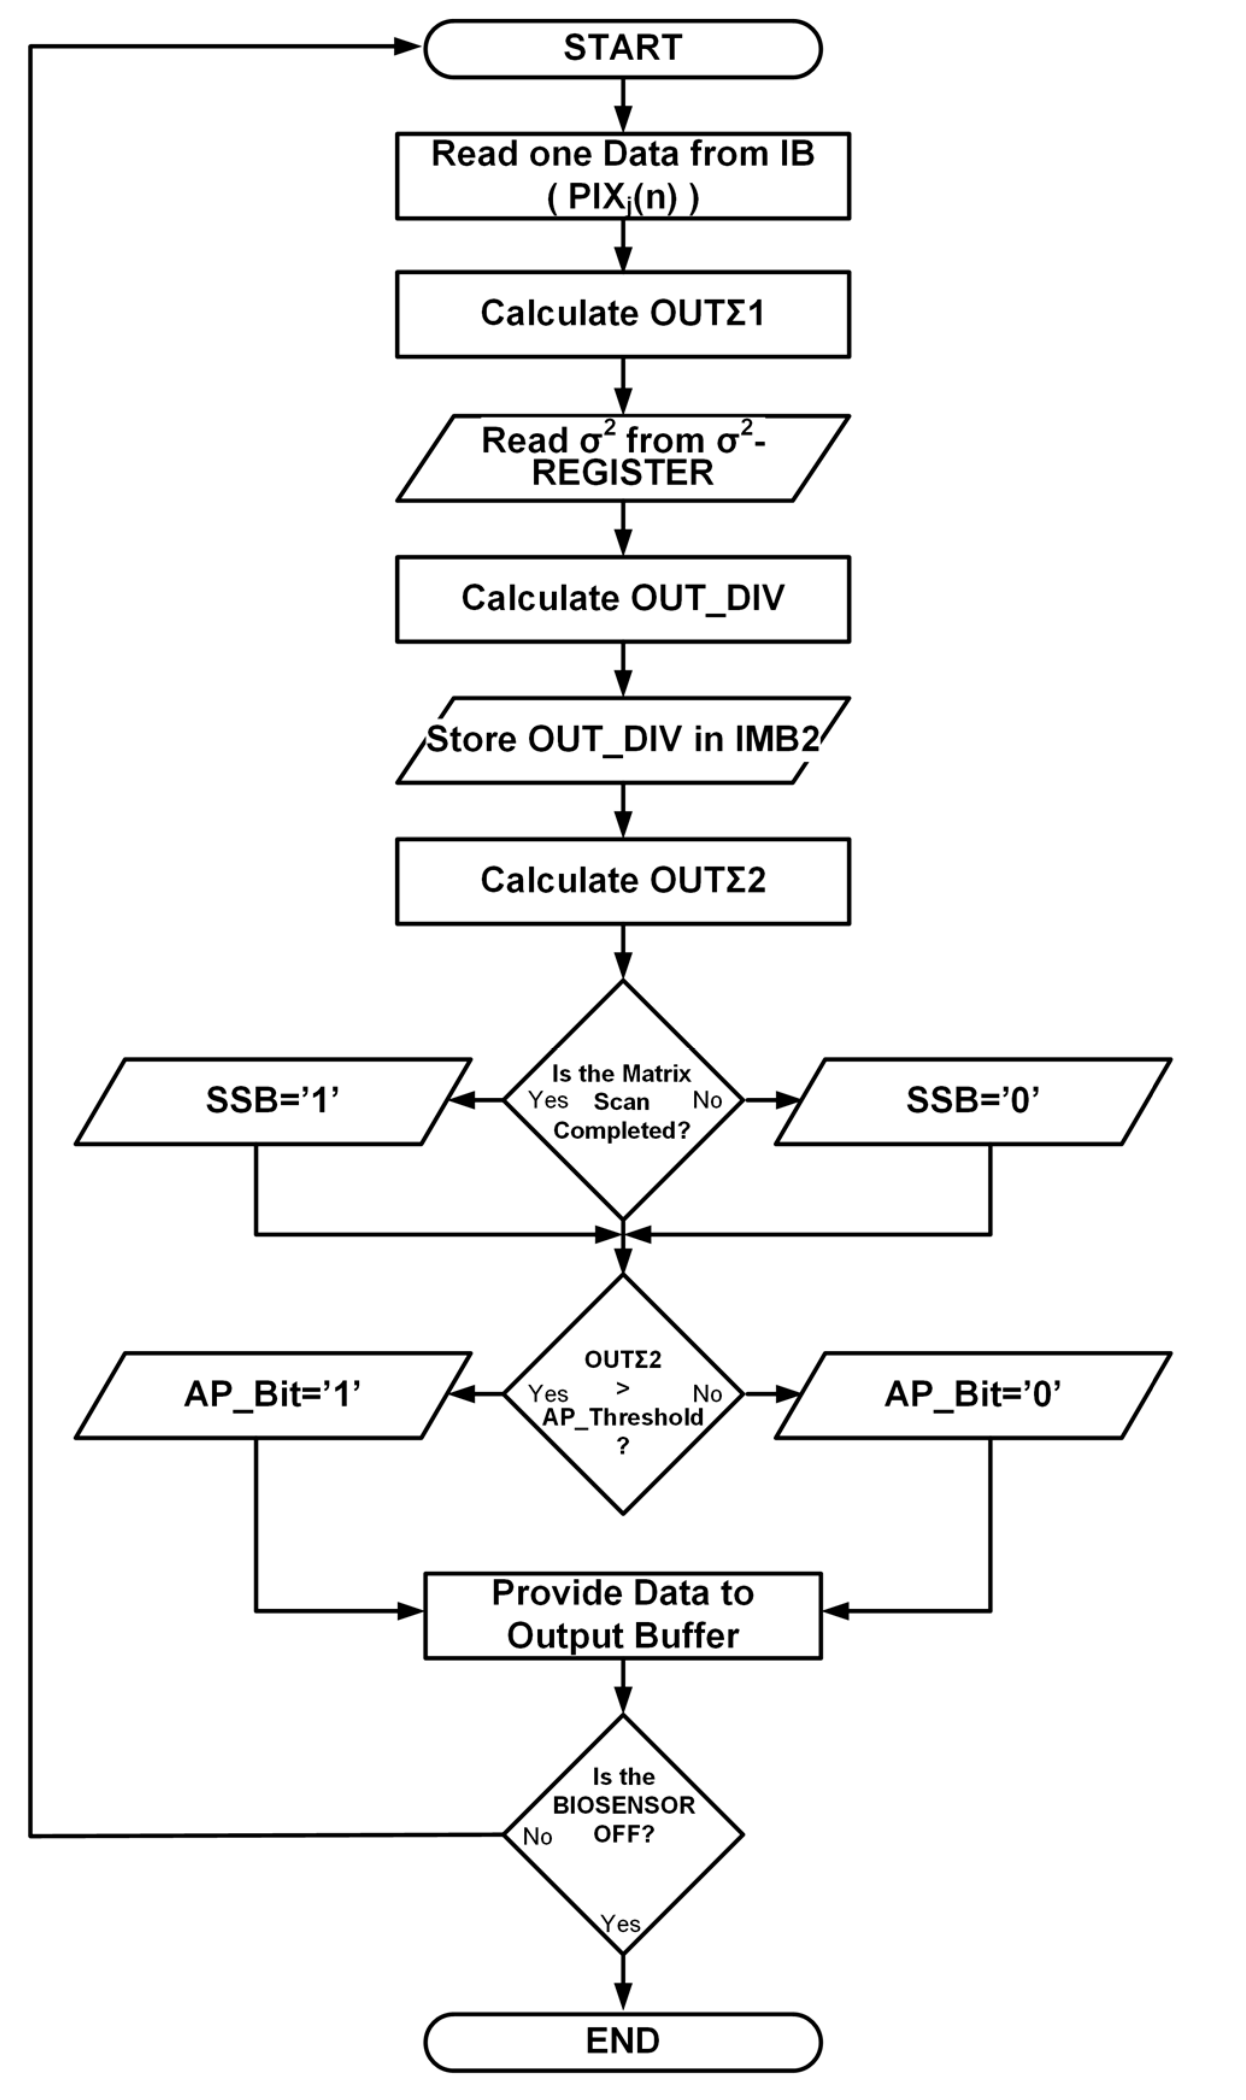
\includegraphics[width=4cm]{PCA_Algorithm.png}
                \caption{PCA algorithm.}
            \end{figure}
        \end{column}
        \hspace{-0.6cm}
        \begin{column}{0.7\textwidth}
            \begin{itemize}
            	\item Each time a new data (PIXj(n)), is received from the MEA, the APD executes the operations illustrated in the flowchart.
                \item The APD performs all the operations that are required to verify the specific condition expressed in Equation:
            \end{itemize}
            \begin{small}
            \begin{equation}
                \sum_{pixj=1\xrightarrow{}9} \frac{\sum_{ \{ n,n-i,n-2 \} } PIXj (n)^2 }{\sigma_{NOISE,j}^2} \geq AP\_Threshold \nonumber
            \end{equation}
            \end{small}
        \end{column}
    \end{columns}
\end{frame}

%%%%%%%%%%%%%%%%%%%%%%%%%%%%%%%%%%%%%%%%%%%%%%%%%%%%%%%%%%%%%%%%%%%%%%%%%%%%%%%%%%%%%%%
\begin{frame}{Output signals} 
\begin{figure}
    \vspace{-0.6cm}
    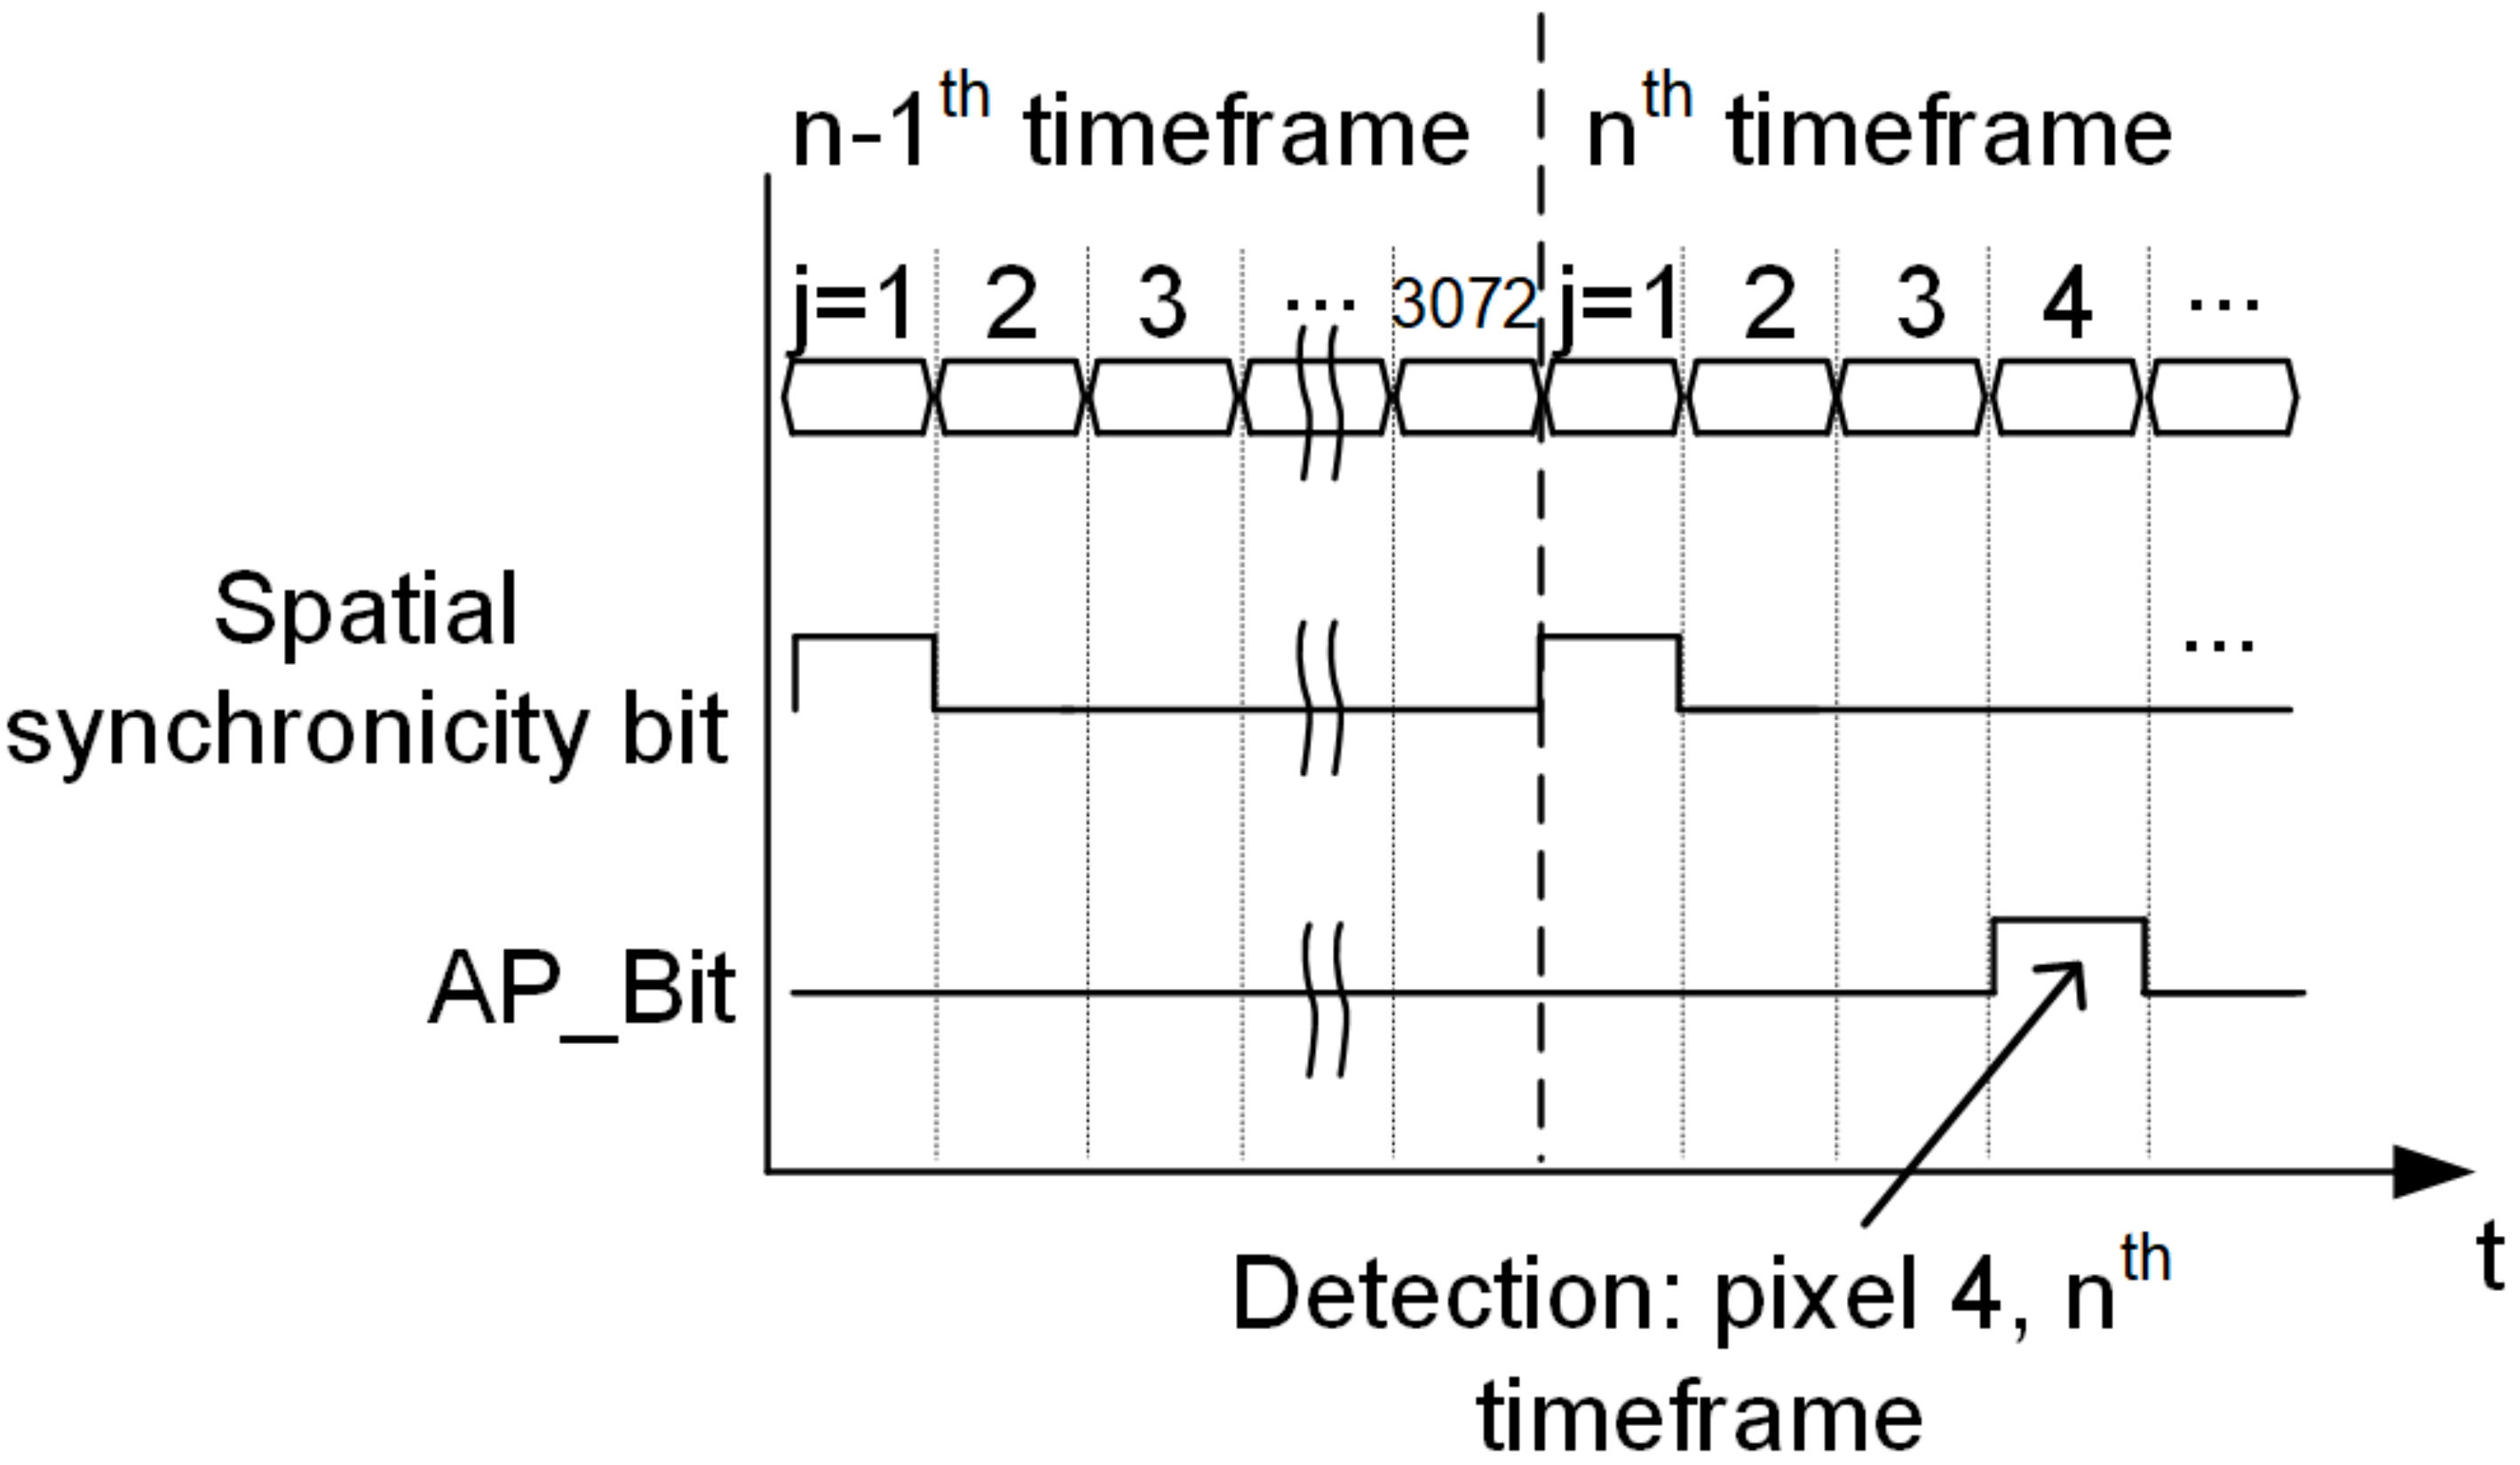
\includegraphics[width=8cm]{bitflag.png}
    \caption{Output signal encoded spatial and temporal information}
\end{figure}
\end{frame}
%%%%%%%%%%%%%%%%%%%%%%%%%%%%%%%%%%%%%%%%%%%%%%%%%%%%%%%%%%%%%%%%%%%%%%%%%%%%%%%%%%%%%%%
\begin{frame}{Output signals} 
\begin{figure}
    \vspace{-0.6cm}
    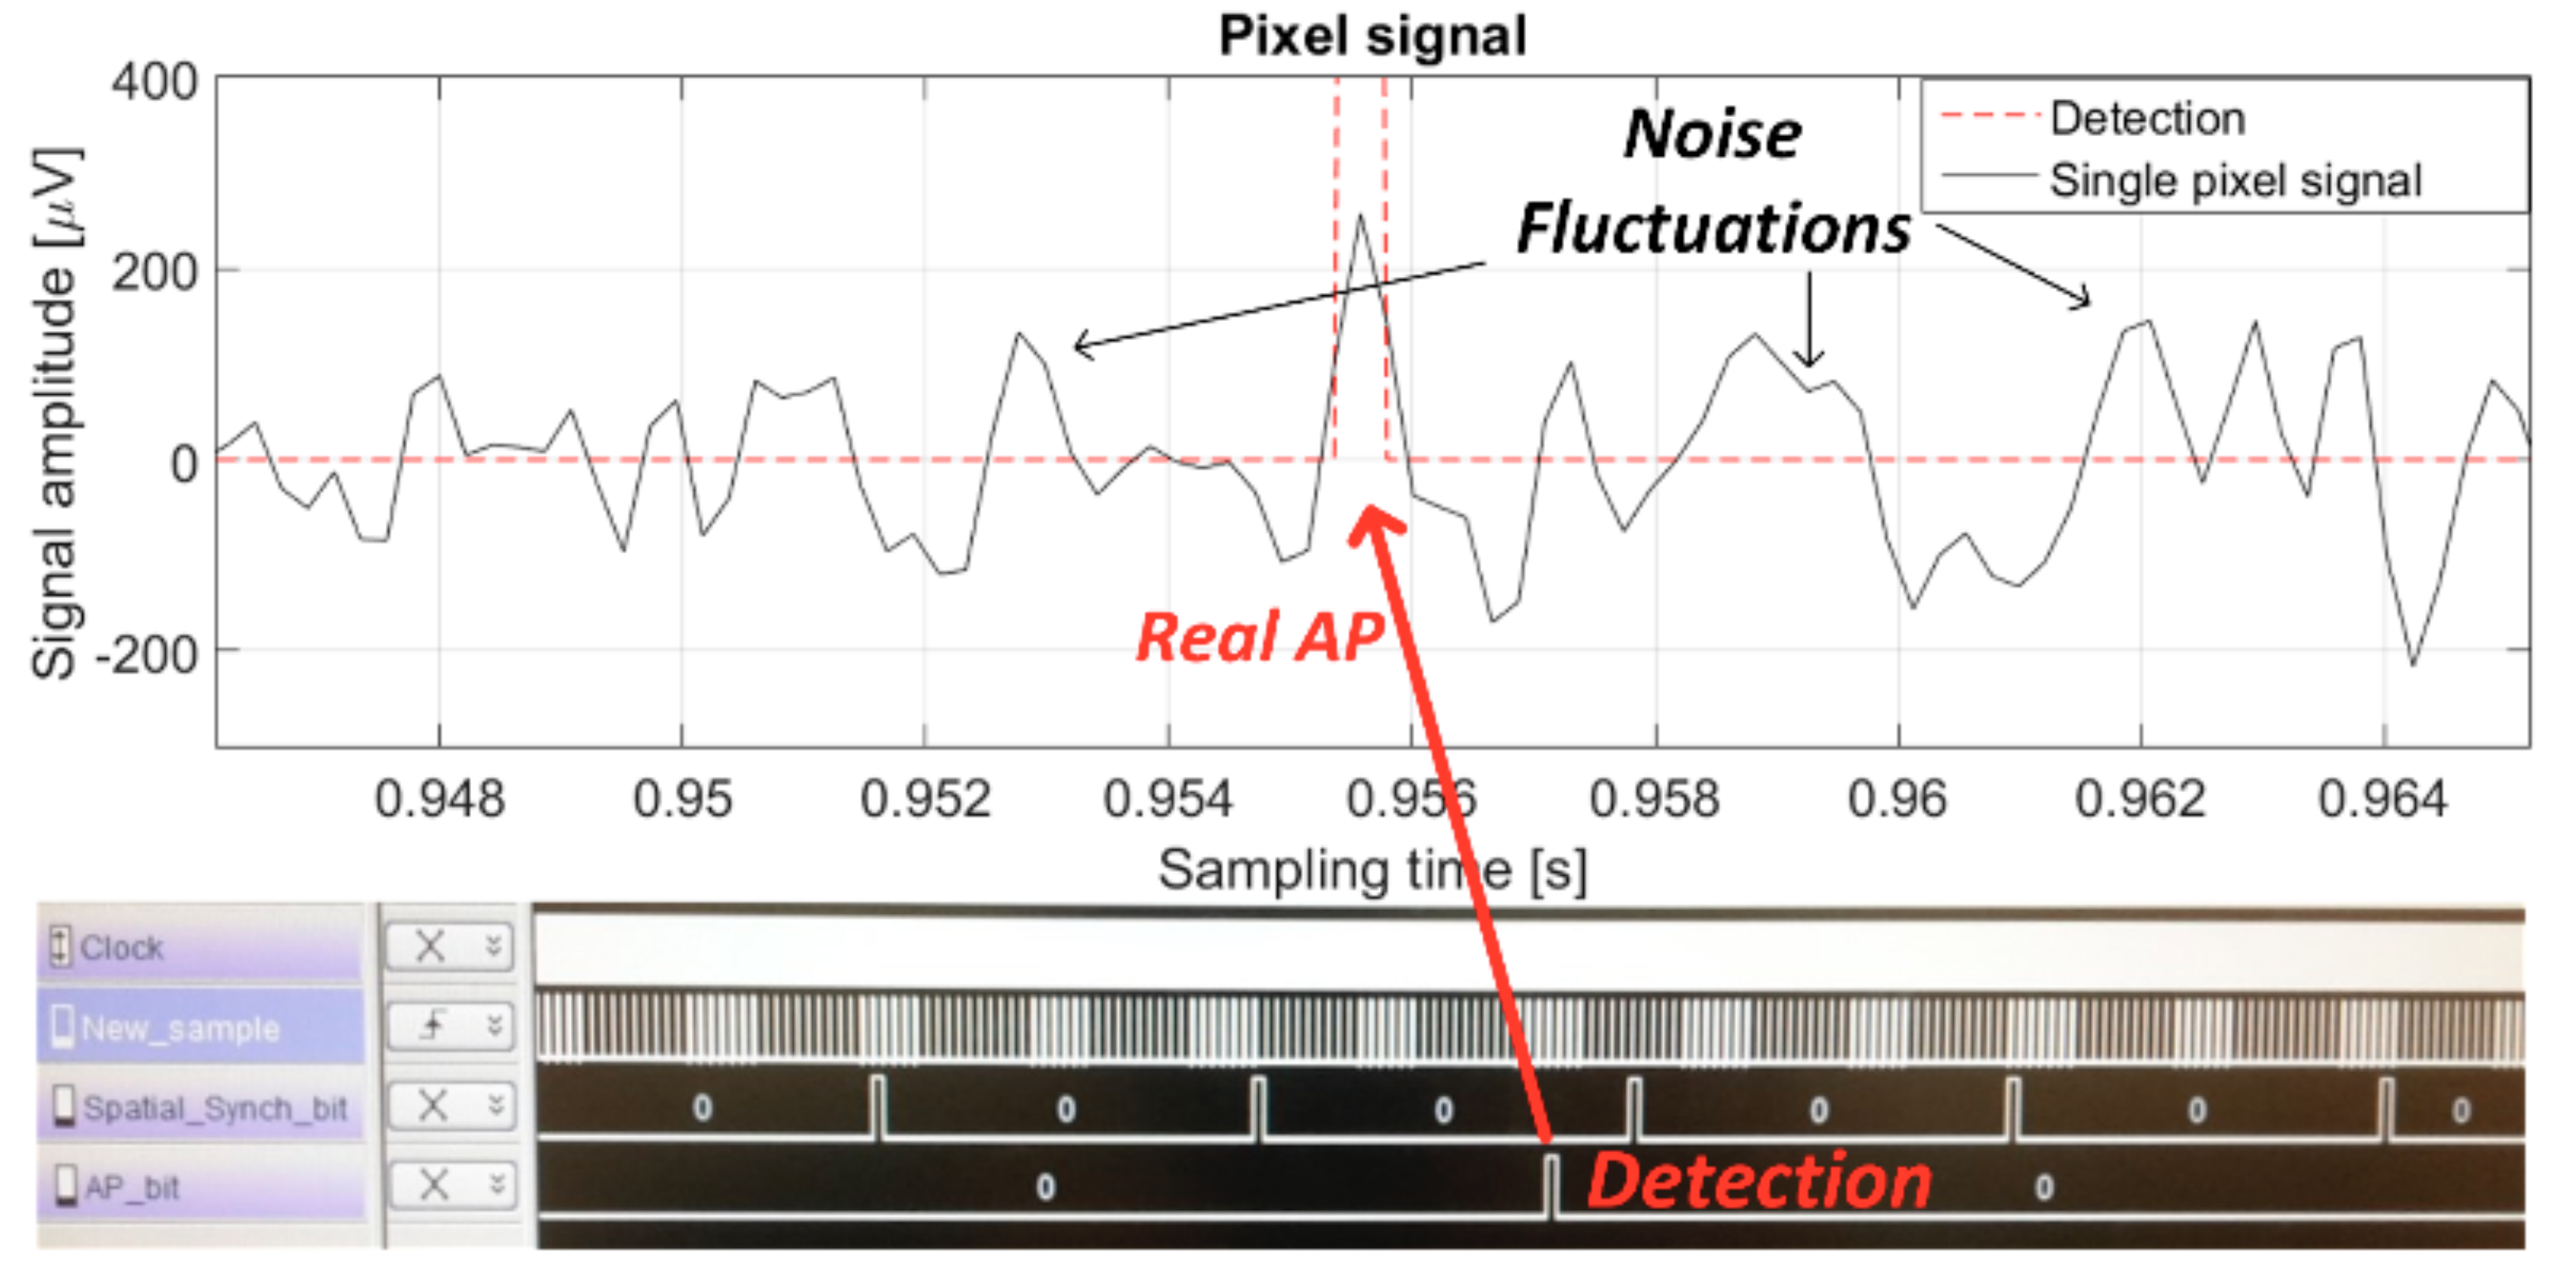
\includegraphics[width=10cm]{Output.png}
    \caption{AP detection and single pixel signal with AP.}
\end{figure}
\end{frame}	









%%%%%%%%%%%%%%%%%%%%%%%%%%%%%%%%%%%%%%%%%%%%%%%%%%%%%%%%%%%%%%%%%%%%%%%%%%%%%%%%%%%%%%%
% ROCCO
%%%%%%%%%%%%%%%%%%%%%%%%%%%%%%%%%%%%%%%%%%%%%%%%%%%%%%%%%%%%%%%%%%%%%%%%%%%%%%%%%%%%%%%

%%%%%%%%%%%%%%%%%%%%%%%%%%%%%%%%%%%%%%%%%%%%%%%%%%%%%%%%%%%%%%%%%%%%%%%%%%%%%%%%%%%%%%%
\begin{frame}{APD FPGA Hardware Implementation} 
    The APD algorithm is implemented by a VHDL digital circuit with:
    \vspace{-5mm}
    \begin{itemize}
        \item \alert{Control Unit} (\textbf{CU});
        \item \alert{Arithmetic Logic Unit} (\textbf{ALU}).
    \end{itemize}
    \begin{figure}
        \centering
        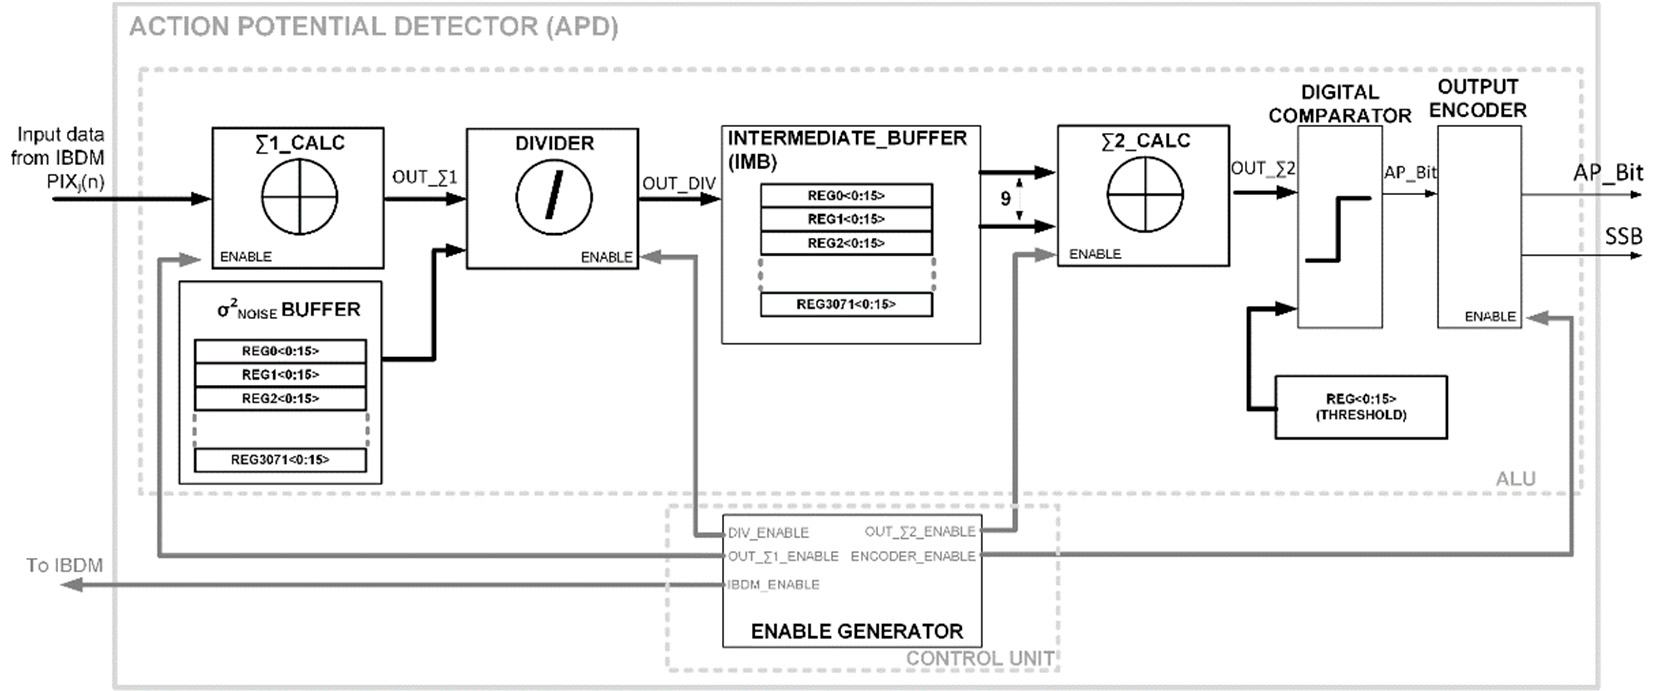
\includegraphics[width=\textwidth]{Images_Rocco/APD_scheme.png}
        \caption{Action Potential Detector (APD) block scheme.}
        \label{fig:AR_APD_scheme}
    \end{figure}
\end{frame}
%%%%%%%%%%%%%%%%%%%%%%%%%%%%%%%%%%%%%%%%%%%%%%%%%%%%%%%%%%%%%%%%%%%%%%%%%%%%%%%%%%%%%%%

%%%%%%%%%%%%%%%%%%%%%%%%%%%%%%%%%%%%%%%%%%%%%%%%%%%%%%%%%%%%%%%%%%%%%%%%%%%%%%%%%%%%%%%
\begin{frame}{APD FPGA Hardware Implementation}
    \framesubtitle{Arithmetic Logic Unit (ALU)}
    \alert{\boxed{\bf ALU}} : arithmetic, logic and memory blocks that perform the operations presented before. Technical details:
    \begin{itemize}
        \item Input data encoded as signed \textbf{14-bit integers}.
        \item Then recoded to \textbf{9-bit resolution}.
        \item The operations are then performed with \textbf{unsigned integer arithmetic}.
        \item After each block of the ALU, data recoded again to the \textbf{minimum needed resolution}.
        \item Computational errors only in the division between integers (\textbf{Radix-2 algorithm}).
        \item To minimize this error, both the numerator and the threshold are multiplied by 256.
    \end{itemize}
\end{frame}
%%%%%%%%%%%%%%%%%%%%%%%%%%%%%%%%%%%%%%%%%%%%%%%%%%%%%%%%%%%%%%%%%%%%%%%%%%%%%%%%%%%%%%%

%%%%%%%%%%%%%%%%%%%%%%%%%%%%%%%%%%%%%%%%%%%%%%%%%%%%%%%%%%%%%%%%%%%%%%%%%%%%%%%%%%%%%%%
\begin{frame}{APD FPGA Hardware Implementation}
    \framesubtitle{Control Unit (CU)}
    \alert{\boxed{\bf CU}} : it regulates the behaviour of the ALU using specific enable signals and spatial pointers, which control the evolution of the algorithm.
    \vspace{1cm}
    \begin{figure}
        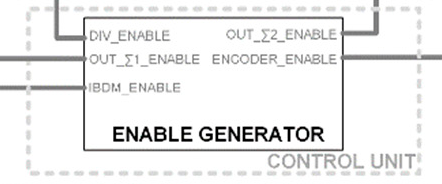
\includegraphics[width=0.5\textwidth]{Images_Rocco/CU.png}
        \caption{Signals of the CU block.}
        \label{fig:AR_CU_time_evolution}
    \end{figure}
\end{frame}
%%%%%%%%%%%%%%%%%%%%%%%%%%%%%%%%%%%%%%%%%%%%%%%%%%%%%%%%%%%%%%%%%%%%%%%%%%%%%%%%%%%%%%%

%%%%%%%%%%%%%%%%%%%%%%%%%%%%%%%%%%%%%%%%%%%%%%%%%%%%%%%%%%%%%%%%%%%%%%%%%%%%%%%%%%%%%%%
\begin{frame}{APD FPGA Hardware Implementation}
    \framesubtitle{Control Unit (CU)}
    \begin{columns}
        \begin{column}{0.55\textwidth}
            \begin{figure}
                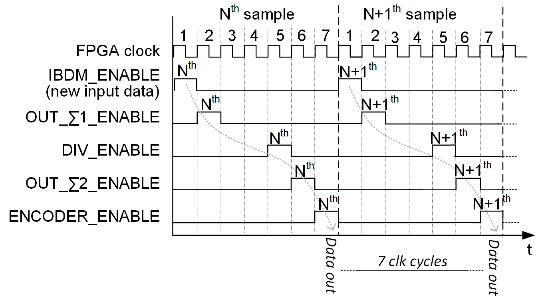
\includegraphics[width=\textwidth]{Images_Rocco/CU_time_evolution.png}
                \caption{Time evolution of CU.}
                \label{fig:AR_CU_time_evolution}
            \end{figure}
        \end{column}
        \hspace{-0.8cm}
        \begin{column}{0.45\textwidth}
            In sequence:
            \begin{enumerate}
            	\item \alert{\bf IBDM\_ENABLE}%high: new data is read from the input buffer in IBDM.
                \item \alert{\bf OUT\_$\Sigma$1\_ENABLE}
                \item \alert{\bf DIV\_ENABLE}
                \item \alert{\bf OUT\_$\Sigma$2\_ENABLE}% progressively and synchronously activated.
                \item \alert{\bf ENCODER\_ENABLE}%: it regulates the timing of the output signals.
            \end{enumerate}
        \end{column}
    \end{columns}
\end{frame}
%%%%%%%%%%%%%%%%%%%%%%%%%%%%%%%%%%%%%%%%%%%%%%%%%%%%%%%%%%%%%%%%%%%%%%%%%%%%%%%%%%%%%%%

%%%%%%%%%%%%%%%%%%%%%%%%%%%%%%%%%%%%%%%%%%%%%%%%%%%%%%%%%%%%%%%%%%%%%%%%%%%%%%%%%%%%%%%
\begin{frame}{APD FPGA Hardware Implementation}
    \framesubtitle{Control Unit (CU)}
    This configuration allows to encode the entire spatial and temporal activity of the biological neuronal net in three single bits:
    \begin{itemize}
        \item \alert{\bf AP\_Bit}: detection information.
        \item \alert{\bf FPGA master clock}: temporal pointer.
        \item \alert{\bf SSB}: spatial pointer.
    \end{itemize}
    Each operation is performed during a single cycle of the FPGA master clock, except the division that lasts three clock cycles.\\
    $\Longrightarrow$ {\bf 7 clock cycles to process a single data}.
\end{frame}
%%%%%%%%%%%%%%%%%%%%%%%%%%%%%%%%%%%%%%%%%%%%%%%%%%%%%%%%%%%%%%%%%%%%%%%%%%%%%%%%%%%%%%%

%%%%%%%%%%%%%%%%%%%%%%%%%%%%%%%%%%%%%%%%%%%%%%%%%%%%%%%%%%%%%%%%%%%%%%%%%%%%%%%%%%%%%%%
\begin{frame}{APD Control Unit Pipeline Approach}
    Input data rate:
    \[
        \text{MEA}_{\mathrm{OUT,RATE}} = 14.1 \ \si{MS/s}
        \overset{\text{7 clk/data}}{\Longrightarrow}
        f_{\mathrm{clk}} = 98.7 \ \si{MHz}
    \]
    It is possible to achieve the same data throughput with a reduced $f_{\mathrm{clk}}$ by using a \alert{\bf pipeline approach}:
    \begin{itemize}
        \item Optimization of the intrinsic parallelization properties of the FPGA.
        \item Technique: provide a new data input to the ALU as soon as the first stage has produced an output.
    \end{itemize}
\end{frame}
%%%%%%%%%%%%%%%%%%%%%%%%%%%%%%%%%%%%%%%%%%%%%%%%%%%%%%%%%%%%%%%%%%%%%%%%%%%%%%%%%%%%%%%

\begin{frame}{APD Control Unit Pipeline Approach}
    \begin{columns}
        \begin{column}{0.5\textwidth}
            \begin{figure}
                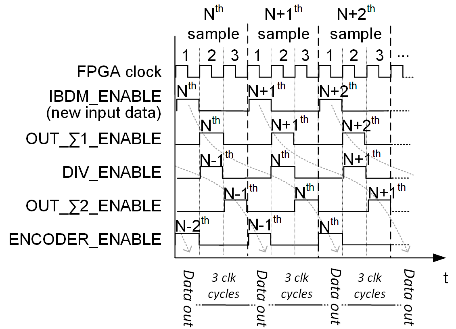
\includegraphics[width=\textwidth]{Images_Rocco/Pipeline.png}
                \caption{Pipelined controller unit enable signals after diagram.}
                \label{fig:AR_Pipeline}
            \end{figure}
        \end{column}
        \hspace{-0.2cm}
        \begin{column}{0.5\textwidth}
            In this way, the system will accept a new input data every three master clock cycles. So:
            \[
                f_{\mathrm{clk}} = 42.3 \ \si{MHz}
            \]
            {\bf Final clock frequency}:
            \[
                \alert{\boxed{f_{\mathrm{clk}} = 42 \ \si{MHz}}}
            \]
        \end{column}
    \end{columns}
\end{frame}
%%%%%%%%%%%%%%%%%%%%%%%%%%%%%%%%%%%%%%%%%%%%%%%%%%%%%%%%%%%%%%%%%%%%%%%%%%%%%%%%%%%%%%%

\begin{frame}{Experimental Results}
NSDD for real-time detection of the neural spikes has been validated by two different setups:
\begin{itemize}
    \item \alert{Behavioral validation}: test-bench $\rightarrow$ check the efficacy of the digital system vs. single pixel SNR.
    
    \item \alert{Biological validation} $\rightarrow$ directly check the NSDD behavior under the signals coming from the CMOS MEA.
\end{itemize}

\end{frame}
%%%%%%%%%%%%%%%%%%%%%%%%%%%%%%%%%%%%%%%%%%%%%%%%%%%%%%%%%%%%%%%%%%%%%%%%%%%%%%%%%%%%%%%

\begin{frame}{Behavioral validation}
\begin{figure}
             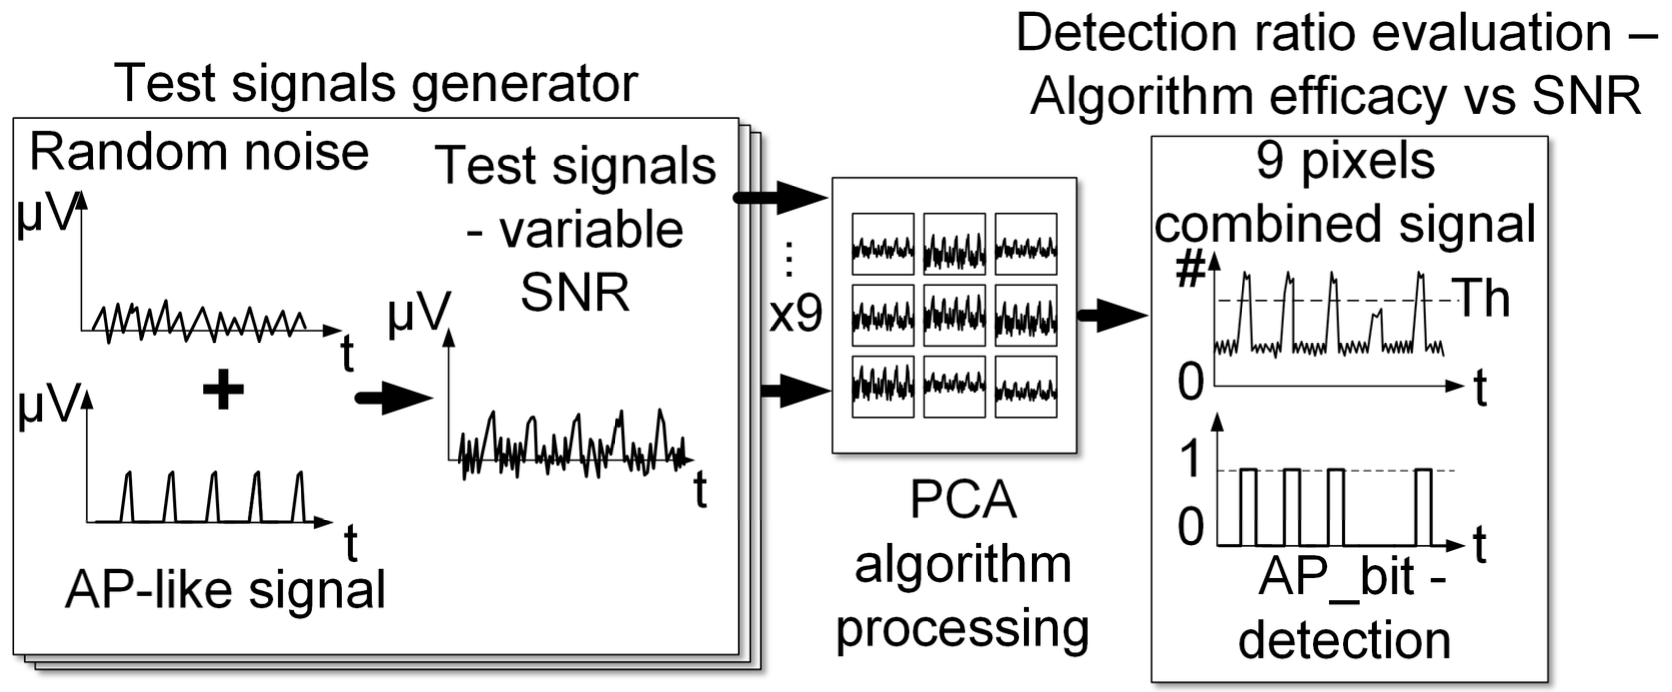
\includegraphics[width=\textwidth]{images_Alice/behavioral_setup.png}
                \caption{Behavioral setup functional scheme.}
                \label{fig:behavioral_setup}
            \end{figure}
\end{frame}
%%%%%%%%%%%%%%%%%%%%%%%%%%%%%%%%%%%%%%%%%%%%%%%%%%%%%%%%%%%%%%%%%%%%%%%%%%%%%%%%%%%%%%%

\begin{frame}{Behavioral validation}
Since the pattern is a priori known, it is possible to \alert{compare} the NSDD output bit with the input pattern.

    \begin{columns}
        \begin{column}{0.6\textwidth}
\begin{figure}
             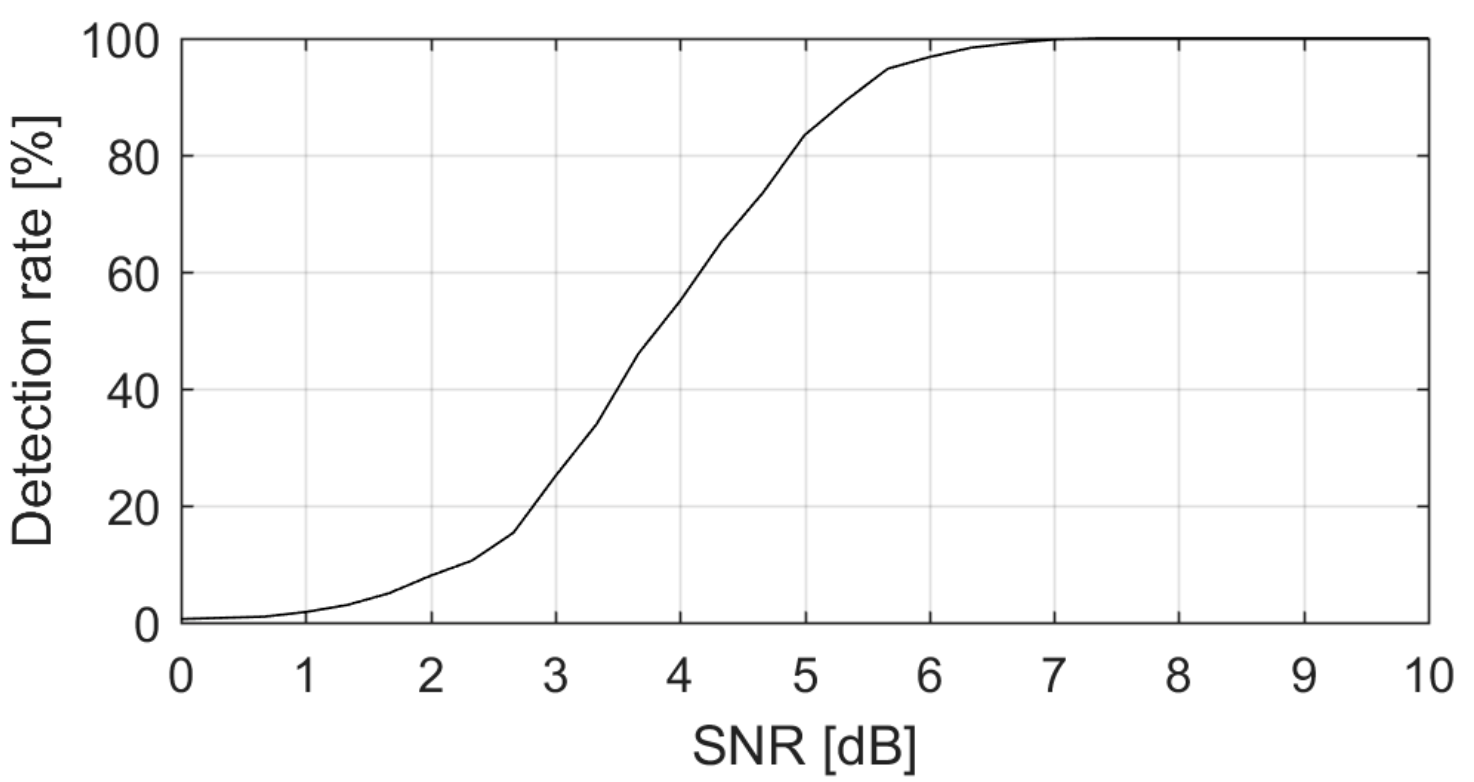
\includegraphics[width=\textwidth]{images_Alice/percent_value.png}
                \caption{Percentage of detected AP versus SNR.}
                \label{fig:behavioral_setup}
            \end{figure}
        \end{column}
        \hspace{-0.2cm}
        \begin{column}{0.4\textwidth}
        
        
        $\Rightarrow$ APs with $250 \mu \text{V}_{\text{0-peak}}$ amplitude are detected with $98\%$ efficacy.
        \vspace{1cm}
\end{column}
\end{columns}
\end{frame}
%%%%%%%%%%%%%%%%%%%%%%%%%%%%%%%%%%%%%%%%%%%%%%%%%%%%%%%%%%%%%%%%%%%%%%%%%%%%%%%%%%%%%%%
\begin{frame}{Biological validation}

NSDD has been tested with the signals coming from the neurons culture. 
\vspace{0.2cm}

The FPGA-APD data allows representing the neuronal cells culture electrical activity by:

\begin{itemize}
    \item neural spike spatial map;
    \item noise power spatial map;
    \item action potential bursting map.
\end{itemize}
\begin{figure}
             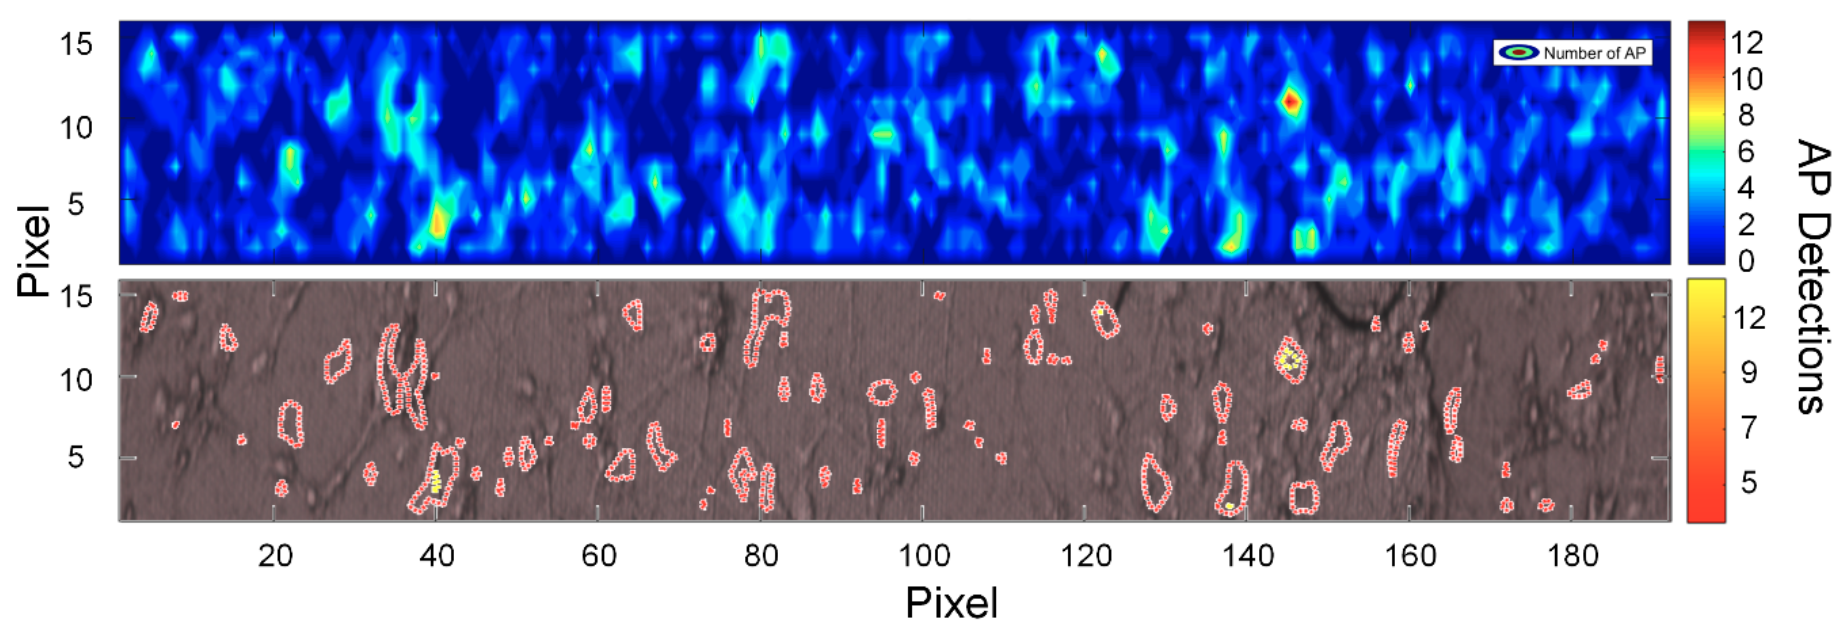
\includegraphics[width=0.65\textwidth]{images_Alice/spatial_map.png}
                \caption{Neural spike (action potential) spatial map.}
                \label{fig:spatial_map}
            \end{figure}
            
\end{frame}
%%%%%%%%%%%%%%%%%%%%%%%%%%%%%%%%%%%%%%%%%%%%%%%%%%%%%%%%%%%%%%%%%%%%%%%%%%%%%%%%%%%%%%%


\begin{frame}{Biological validation}

AP$\_$Bit encodes the detection information (spatial and temporal):
\begin{itemize}
    \item it can be processed to perform spatial and temporal mapping of the APs above the MEA.
    \item it enables event-driven communication and/or it can be used for instantaneous control of the electrical stimulation signal;
\end{itemize}

\end{frame}
%%%%%%%%%%%%%%%%%%%%%%%%%%%%%%%%%%%%%%%%%%%%%%%%%%%%%%%%%%%%%%%%%%%%%%%%%%%%%%%%%%%%%%%



\begin{frame}{Action Potential Bursting}
AP$\_$Bit can be used to detect whether any synchronous activity of the neuron population is happening at any given moment. 

\begin{figure}
             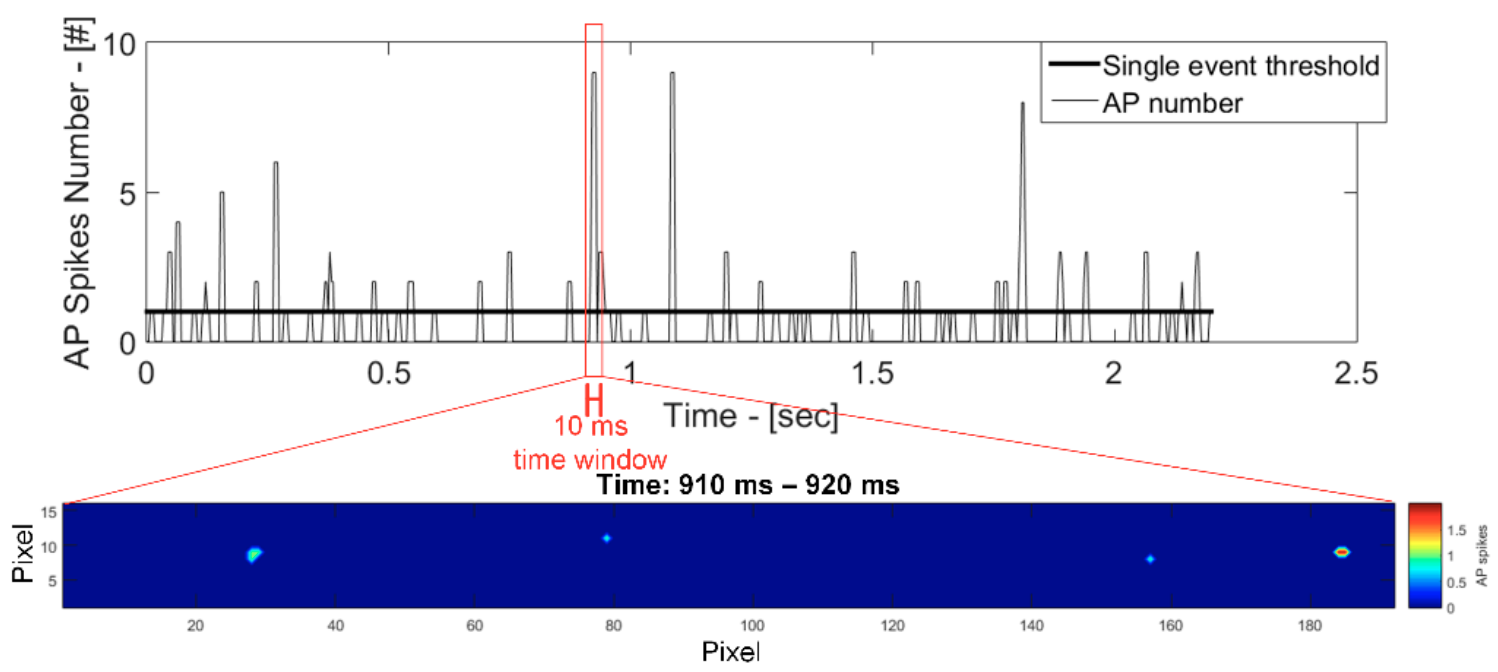
\includegraphics[width=0.85\textwidth]{images_Alice/action_potential_bursting.png}
                \caption{Neuronal spikes map of action potential bursting.}
                \label{fig:action_potential_bursting}
            \end{figure}
            

\end{frame}
%%%%%%%%%%%%%%%%%%%%%%%%%%%%%%%%%%%%%%%%%%%%%%%%%%%%%%%%%%%%%%%%%%%%%%%%%%%%%%%%%%%%%%%
\begin{frame}{Conclusions}
Design of a \alert{complete FPGA-based} circuit:
\begin{itemize}
    \item \alert{monitors} the electrical activity of a hippocampal neuronal cells culture over a micro-electrode array;
    \item \alert{detects} action potentials from background noise.
\end{itemize}
The system is composed by:
\begin{itemize}
    \item VHDL-based FPGA design;
    \item set of MATLAB functions for data evalutation.
\end{itemize}

\end{frame}
%%%%%%%%%%%%%%%%%%%%%%%%%%%%%%%%%%%%%%%%%%%%%%%%%%%%%%%%%%%%%%%%%%%%%%%%%%%%%%%%%%%%%%%
\begin{frame}{Conclusions}
The system implementation allows:
\begin{itemize}
    \item real-time detection;
    \item encoding temporal and spatial information.
\end{itemize}
\vspace{0.5cm}

It has been experimentally validated by producing a spatial map of the on-going electrical activity, which is consistent with spontaneous neural activity rates.
\vspace{0.5cm}

Finally, the output bit-stream has beens used to detect AP bursting events.


\end{frame}
%%%%%%%%%%%%%%%%%%%%%%%%%%%%%%%%%%%%%%%%%%%%%%%%%%%%%%%%%%%%%%%%%%%%%%%%%%%%%%%%%%%%%%%

\begin{frame}
\it{\LARGE Grazie per l'attenzione.}		
\end{frame}

%%%%%%%%%%%%%%%%%%%%%%%%%%%%%%%%%%%%%%%%%%%%%%%%%%%%%%%%%%%%%%%%%%%%%%%%%%%%%%%%%%%%%%%



\end{document}

